\documentclass[tikz,border=10pt]{standalone}\usepackage{tikz}\usetikzlibrary{arrows.meta,positioning}\begin{document}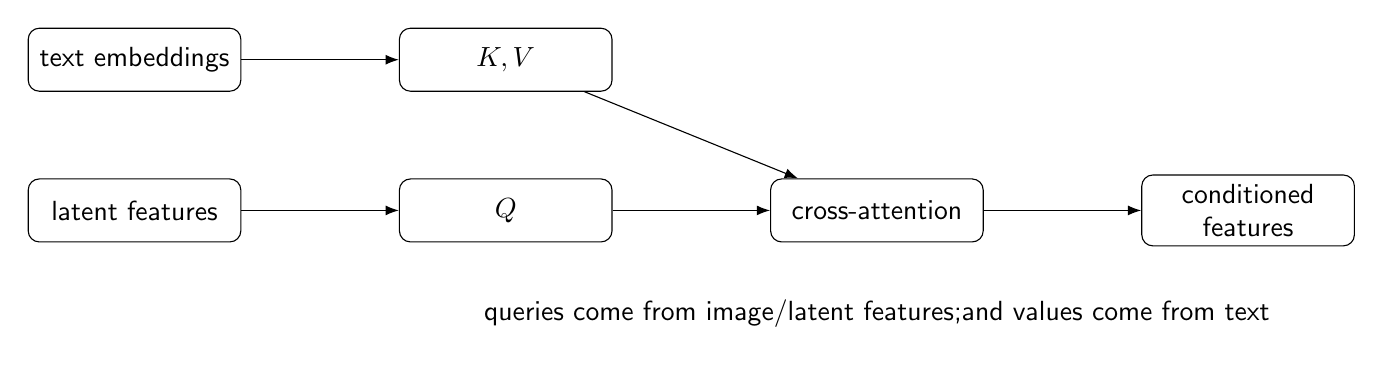
\begin{tikzpicture}[font=\sffamily,>=Latex,box/.style={draw,rounded corners,align=center,minimum width=2.7cm,minimum height=.8cm}]\node[box](lat){latent features};\node[box,above=1.1cm of lat](text){text embeddings};\node[box,right=2cm of lat](q){$Q$};\node[box,right=2cm of text](kv){$K, V$};\node[box,right=2cm of q](att){cross-attention};\node[box,right=2cm of att](out){conditioned\\features};\draw[->](lat)--(q);\draw[->](text)--(kv);\draw[->](q)--(att);\draw[->](kv)--(att);\draw[->](att)--(out);\node[below=.6cm of att,align=center]{queries come from image/latent features;\keys and values come from text};\end{tikzpicture}\end{document}
